\chapter{Analisis}
\label{chap:analisis}

Bab ini membahas tentang analisis cara kerja algoritma \textit{backtracking} dan algoritma \textit{hybrid genetic} untuk menyelesaikan permainan teka-teki Calcudoku, dan analisis kebutuhan perangkat lunak Calcudoku.

\section{Analisis Algoritma \textit{Backtracking}}
\label{sec:analisisbt}

Untuk mengilustrasikan cara kerja algoritma \textit{backtracking}, akan digunakan permainan teka-teki Calcudoku yang digambarkan pada Gambar~\ref{fig:analisisbt1} sebagai contoh.

\begin{figure}
\centering
\captionsetup{justification=centering}
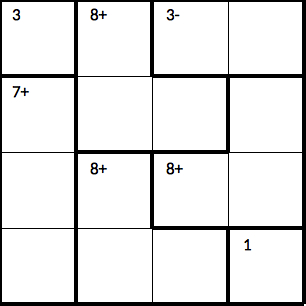
\includegraphics[scale=0.333]{Gambar/backtracking/State1}
\caption[Contoh permainan teka-teki Calcudoku dengan ukuran \textit{grid} 4 x 4 yang belum diselesaikan, seperti yang digambarkan pada Gambar~\ref{fig:backtracking1}.  ~\cite{fahda:16:backtracking}]{Contoh permainan teka-teki dengan ukuran \textit{grid} 4 x 4 yang belum diselesaikan, seperti yang digambarkan pada Gambar~\ref{fig:backtracking1}.  ~\cite{fahda:16:backtracking}}
\label{fig:analisisbt1}
\end{figure}

\begin{enumerate}
\item Algoritma \textit{backtracking} dimulai dengan teka-teki yang belum diselesaikan, seperti yang digambarkan pada Gambar~\ref{fig:analisisbt1} (\textit{state} 1).
\item Algoritma mengisikan sel pada baris ke-1 dan kolom ke-1 dengan angka 1 (\textit{state} 2), tetapi angka 1 tidak sesuai dengan angka tujuan dari \textit{cage} tersebut.
\item Algoritma lalu mencoba kemungkinan angka berikutnya, yaitu angka 2 (\textit{state} 3), tetapi angka 2 juga tidak sesuai dengan angka tujuan dari \textit{cage} tersebut.
\item Algoritma lalu mencoba kemungkinan angka berikutnya, yaitu angka 3 (\textit{state} 4), seperti dapat dilihat pada Gambar~\ref{fig:analisisbt2}, dan ternyata angka 3 sesuai dengan angka tujuan dari \textit{cage} tersebut, sehingga algoritma dapat maju ke sel berikutnya.

\begin{figure}
\centering
\captionsetup{justification=centering}
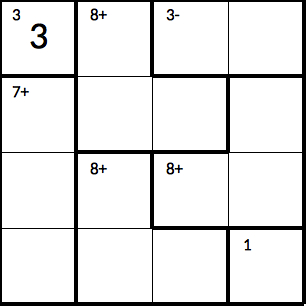
\includegraphics[scale=0.333]{Gambar/backtracking/State4}
\caption[\textit{State} 4]{\textit{State} 4}
\label{fig:analisisbt2}
\end{figure}

\item Algoritma lalu mengisikan sel pada baris ke-1 dan kolom ke-2 dengan angka 1 (\textit{state} 5). Algoritma lalu maju ke sel berikutnya.
\item Algoritma lalu mengisikan sel pada baris ke-1 dan kolom ke-3 dengan angka 1 (\textit{state} 6), tetapi angka 1 sudah pernah digunakan dalam baris tersebut.
\item Algoritma lalu mencoba kemungkinan angka berikutnya, yaitu angka 2 (\textit{state} 7). Algoritma lalu maju ke sel berikutnya.
\item Algoritma lalu mengisikan sel pada baris ke-1 dan kolom ke-4 dengan angka 1 (\textit{state} 8), tetapi angka 1 sudah pernah digunakan dalam baris tersebut.
\item Algoritma lalu mencoba kemungkinan angka berikutnya, yaitu angka 2 (\textit{state} 9), tetapi angka 2 sudah pernah digunakan dalam baris tersebut.
\item Algoritma lalu mencoba kemungkinan angka berikutnya, yaitu angka 3 (\textit{state} 10), tetapi angka 3 sudah pernah digunakan dalam baris tersebut.
\item Algoritma lalu mencoba kemungkinan angka berikutnya, yaitu angka 4 (\textit{state} 11), seperti dapat dilihat pada Gambar~\ref{fig:analisisbt3}, tetapi hasilnya tidak sesuai dengan angka tujuan dari \textit{cage} tersebut.

\begin{figure}
\centering
\captionsetup{justification=centering}
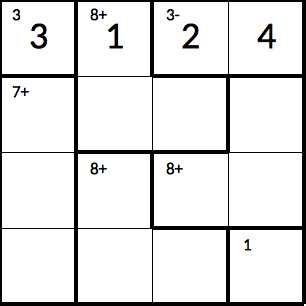
\includegraphics[scale=0.333]{Gambar/backtracking/State11}
\caption[\textit{State} 11]{\textit{State} 11}
\label{fig:analisisbt3}
\end{figure}

\item Karena semua kemungkinan angka untuk baris ke-1 dan kolom ke-4 telah dicoba dan gagal, maka algoritma harus mundur kembali ke (\textit{state} 7). Algoritma mencoba kemungkinan angka berikutnya, yaitu angka 3  (\textit{state} 12), seperti dapat dilihat pada Gambar~\ref{fig:analisisbt4}, tetapi angka 3 sudah pernah digunakan dalam baris tersebut.

\begin{figure}
\centering
\captionsetup{justification=centering}
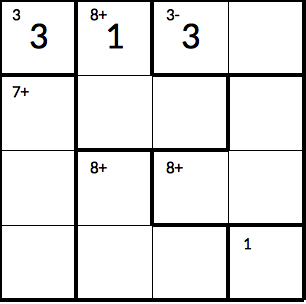
\includegraphics[scale=0.333]{Gambar/backtracking/State12}
\caption[\textit{State} 12]{\textit{State} 12}
\label{fig:analisisbt4}
\end{figure}

\item Algoritma lalu mencoba kemungkinan angka berikutnya, yaitu angka 4 (\textit{state} 13). Algoritma lalu maju ke sel berikutnya.
\item Algoritma lalu mengisikan sel pada baris ke-1 dan kolom ke-4 dengan angka 1 (\textit{state} 14), tetapi angka 1 sudah pernah digunakan dalam baris tersebut.
\item Algoritma lalu mencoba kemungkinan angka berikutnya, yaitu angka 2 (\textit{state} 15), tetapi hasilnya tidak sesuai dengan angka tujuan dari \textit{cage} tersebut.
\item Algoritma lalu mencoba kemungkinan angka berikutnya, yaitu angka 3 (\textit{state} 16), tetapi angka 3 sudah pernah digunakan dalam baris tersebut.
\item Algoritma lalu mencoba kemungkinan angka berikutnya, yaitu angka 4 (\textit{state} 17), seperti dapat dilihat pada Gambar~\ref{fig:analisisbt5}, tetapi angka 4 sudah pernah digunakan dalam baris tersebut.

\begin{figure}
\centering
\captionsetup{justification=centering}
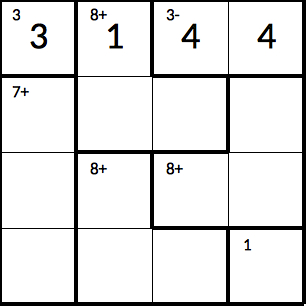
\includegraphics[scale=0.333]{Gambar/backtracking/State17}
\caption[\textit{State} 17]{\textit{State} 17}
\label{fig:analisisbt5}
\end{figure}

\item Karena semua kemungkinan angka untuk baris ke-1 dan kolom ke-3 dan ke-4 telah dicoba dan gagal, maka algoritma harus mundur kembali ke (\textit{state} 5). Algoritma mencoba kemungkinan angka berikutnya, yaitu angka 2  (\textit{state} 18), seperti dapat dilihat pada Gambar~\ref{fig:analisisbt6}. Algoritma lalu maju ke sel berikutnya.

\begin{figure}
\centering
\captionsetup{justification=centering}
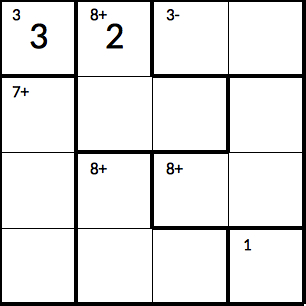
\includegraphics[scale=0.333]{Gambar/backtracking/State18}
\caption[\textit{State} 18]{\textit{State} 18}
\label{fig:analisisbt6}
\end{figure}

\item Algoritma lalu mengisikan sel pada baris ke-1 dan kolom ke-3 dengan angka 1 (\textit{state} 19), seperti dapat dilihat pada Gambar~\ref{fig:analisisbt7}. Algoritma lalu maju ke sel berikutnya.

\begin{figure}
\centering
\captionsetup{justification=centering}
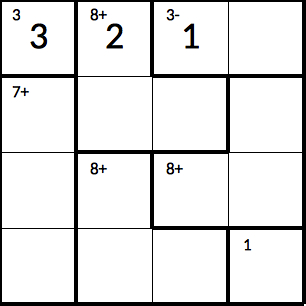
\includegraphics[scale=0.333]{Gambar/backtracking/State19}
\caption[\textit{State} 19]{\textit{State} 19}
\label{fig:analisisbt7}
\end{figure}

\item Algoritma lalu mengisikan sel pada baris ke-1 dan kolom ke-4 dengan angka 1 (\textit{state} 20), tetapi angka 1 sudah pernah digunakan dalam baris tersebut.
\item Algoritma lalu mencoba kemungkinan angka berikutnya, yaitu angka 2 (\textit{state} 21), tetapi angka 2 sudah pernah digunakan dalam baris tersebut.
\item Algoritma lalu mencoba kemungkinan angka berikutnya, yaitu angka 3 (\textit{state} 22), tetapi angka 3 sudah pernah digunakan dalam baris tersebut.
\item Algoritma lalu mencoba kemungkinan angka berikutnya, yaitu angka 4 (\textit{state} 23), dan ternyata hasilnya sesuai dengan angka tujuan dari \textit{cage} tersebut, seperti dapat dilihat pada Gambar~\ref{fig:analisisbt8}. Algoritma telah selesai mengisikan baris ke-1, sehingga bisa maju ke baris berikutnya.

\begin{figure}
\centering
\captionsetup{justification=centering}
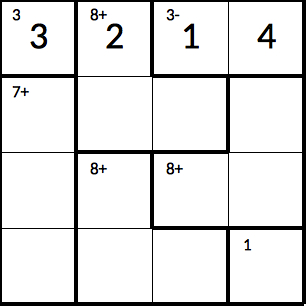
\includegraphics[scale=0.333]{Gambar/backtracking/State23}
\caption[\textit{State} 23]{\textit{State} 23}
\label{fig:analisisbt8}
\end{figure}

\item Langkah-langkah di atas diulang untuk mengisi sel-sel pada baris-baris selanjutnya. Algoritma \textit{backtracking} berhasil mengisi semua sel dalam permainan teka-teki Calcudoku ini dengan benar pada \textit{state} 93, seperti dapat dilihat pada Gambar~\ref{fig:analisisbt32}.

\begin{figure}
\centering
\captionsetup{justification=centering}
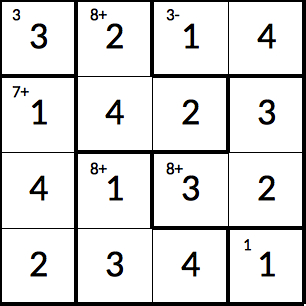
\includegraphics[scale=0.333]{Gambar/backtracking/State93}
\caption[\textit{State} 93]{\textit{State} 93}
\label{fig:analisisbt32}
\end{figure}

\end{enumerate}

Algoritma ini mencapai solusinya pada state 93, seperti pada \textit{state space tree} yang digambarkan dalam Gambar~\ref{fig:analisisbt33}. \textit{State space tree} ini telah mencapai simpul tujuannya, yaitu simpul 93, dengan jalur 3-2-1-4-1-4-2-3-4-1-3-2-2-3-4-1. Penjelasan tentang analisis algoritma \textit{backtracking} secara lengkap dapat dilihat di Lampiran~\ref{chap:analisisbacktracking}.

\begin{landscape}
\begin{figure}
\centering
\captionsetup{justification=centering}
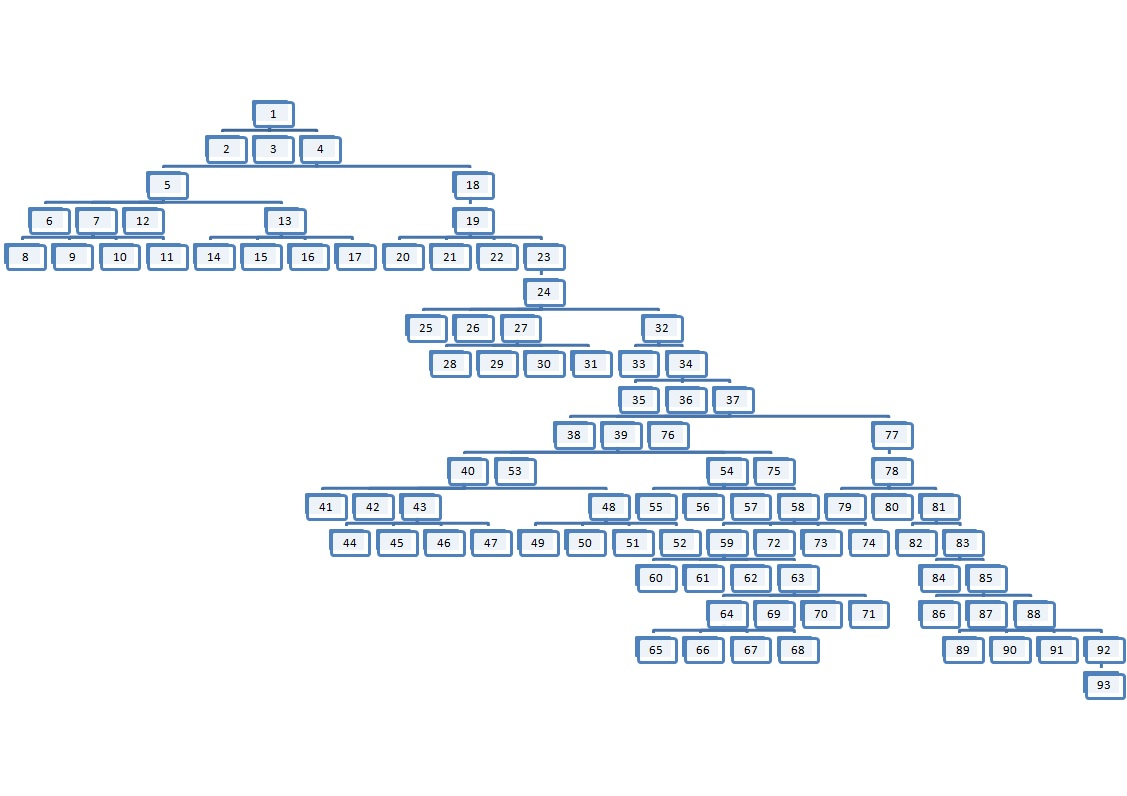
\includegraphics[scale=0.75]{Gambar/backtracking/StateSpaceTree}
\caption[\textit{State space tree} yang dikembangkan dalam proses menyelesaikan teka-teki Calcudoku yang digambarkan pada Gambar~\ref{fig:analisisbt1}]{\textit{State space tree} yang dikembangkan dalam proses menyelesaikan teka-teki Calcudoku yang digambarkan pada Gambar~\ref{fig:analisisbt1}}
\label{fig:analisisbt33}
\end{figure}
\end{landscape}

\section{Analisis Algoritma \textit{Hybrid Genetic}}
\label{sec:analisishg}

Untuk mengilustrasikan cara kerja algoritma \textit{hybrid genetic}, akan digunakan permainan teka-teki Calcudoku yang digambarkan pada Gambar~\ref{fig:analisishg1} sebagai contoh. Algoritma \textit{hybrid genetic} dimulai dengan mencoba menyelesaikan permainan teka-teki Calcudoku dengan algoritma \textit{rule based}.

\begin{figure}
\centering
\captionsetup{justification=centering}
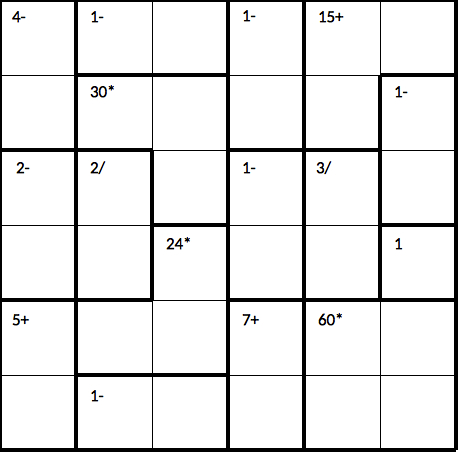
\includegraphics[scale=0.333]{Gambar/hybridgenetic/Puzzle}
\caption[Contoh permainan teka-teki Calcudoku dengan ukuran \textit{grid} 6 x 6 yang belum diselesaikan, seperti yang digambarkan pada Gambar~\ref{fig:hybrid1}. \cite{johanna:12:hybrid}]{Contoh permainan teka-teki Calcudoku dengan ukuran \textit{grid} 6 x 6 yang belum diselesaikan, seperti yang digambarkan pada Gambar~\ref{fig:hybrid1}. \cite{johanna:12:hybrid}}
\label{fig:analisishg1}
\end{figure}

\subsection{Algoritma \textit{Rule Based}}
\label{sec:analisisrb}

Sel pada baris ke-4 dan kolom ke-6 adalah bagian dari sebuah \textit{cage} yang berukuran hanya 1 sel, dan oleh karena itu, angka tujuan dari sel tersebut adalah angka tujuan dari \textit{cage} tersebut (aturan \textit{single square}). Angka tujuan dari \textit{cage} tersebut adalah 1, dan oleh karena itu sel tersebut dapat langsung diisi dengan angka 1, seperti dapat dilihat pada Gambar~\ref{fig:analisishg2}.

Sayangnya, algoritma \textit{rule based} gagal dalam mengisi sel-sel lainnya berdasarkan aturan-aturan yang telah didefinisikan setelah beberapa kali percobaan, sehingga algoritma \textit{hybrid genetic} akan mencoba menyelesaikan teka-teki Calcudoku dengan algoritma genetik.

\begin{figure}
\centering
\captionsetup{justification=centering}
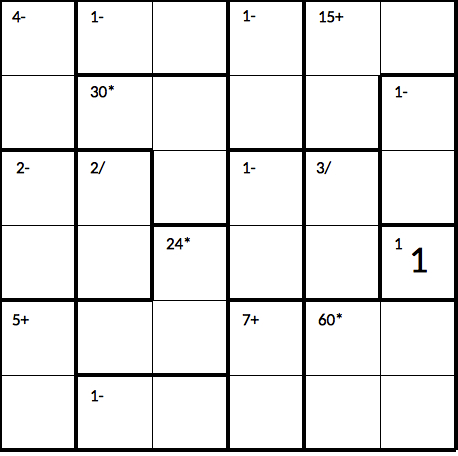
\includegraphics[scale=0.333]{Gambar/hybridgenetic/PuzzleAfterRuleBased}
\caption[Permainan teka-teki Calcudoku setelah diselesaikan dengan algoritma \textit{rule based}]{Permainan teka-teki Calcudoku setelah diselesaikan dengan algoritma \textit{rule based}}
\label{fig:analisishg2}
\end{figure}

\subsection{Algoritma Genetik}
\label{sec:analisisgenetik}

Dalam contoh ini, parameter-parameter untuk algoritma genetik yang akan digunakan untuk teka-teki Calcudoku ini ditunjukkan pada Tabel~\ref{tab:analisishg1}. Dalam kasus ini, parameter ditentukan oleh pembuat program (penulis). Setiap generasi terdiri dari 12 kromosom. \begin{math}40\% \times 12 \approx 5\end{math} kromosom diambil dari generasi sebelumnya (\textit{elitism}). \begin{math}50\% \times 12 \approx 6\end{math} kromosom adalah hasil dari pembentukan kromosom-kromosom baru dengan operasi kawin silang, dan \begin{math}10\% \times 12 \approx 1\end{math} kromosom adalah hasil dari pembentukan kromosom-kromosom baru dengan operasi mutasi. Untuk mengilustrasikan cara kerja algoritma genetik, hanya 3 generasi pertama yang akan dibahas.

Setiap sel mempunyai nilai kelayakan. Nilai kelayakan dari sebuah sel akan bernilai 1 jika nilai dari semua sel yang merupakan bagian dari \textit{cage} yang salah satu selnya adalah sel tersebut menghasilkan nilai tujuan setelah dihitung menggunakan operator yang telah ditentukan dan tidak ada pengulangan angka di dalam baris tersebut maupun kolom tersebut, dan bernilai 0 jika nilai dari semua sel yang merupakan bagian dari \textit{cage} yang salah satu selnya adalah sel tersebut tidak menghasilkan nilai tujuan setelah dihitung menggunakan operator yang telah ditentukan atau ada pengulangan angka di dalam baris tersebut maupun kolom tersebut. Nilai kelayakan sel untuk setiap sel dalam sebuah baris dijumlahkan, lalu dibagi dengan jumlah kolom dalam baris tersebut, dan hasilnya adalah nilai kelayakan baris. Nilai kelayakan baris untuk setiap baris dalam sebuah teka-teki dijumlahkan, lalu dibagi dengan jumlah baris dalam teka-teki tersebut, dan hasilnya adalah nilai kelayakan teka-teki.

\begin{table}
\centering
\captionsetup{justification=centering}
\caption[Tabel parameter untuk algoritma genetik yang akan digunakan untuk menyelesaikan teka-teki Calcudoku yang digambarkan pada Gambar~\ref{fig:analisishg2}]{Tabel parameter untuk algoritma genetik yang akan digunakan untuk menyelesaikan teka-teki Calcudoku yang digambarkan pada Gambar~\ref{fig:analisishg2}}
\begin{tabular}{| l | l |}
\hline
Parameter & Nilai \\
\hline \hline
Ukuran Populasi & 12 \\
\hline
Probabilitas \textit{Elitism} & 40\% \\
\hline
Probabilitas Kawin Silang & 50\% \\
\hline
Probabilitas Mutasi & 10\% \\
\hline
\end{tabular}
\label{tab:analisishg1}
\end{table}

Algoritma genetik dimulai dengan membangkitkan kromosom-kromosom baru sebanyak ukuran populasi yang telah ditentukan. Dalam contoh ini, ukuran populasi adalah 12, maka algoritma akan membangkitkan 12 kromosom baru. Ke-12 kromosom awal ini adalah bagian dari generasi pertama. Gambar~\ref{fig:analisisg1k1} menggambarkan Kromosom 1, gambar~\ref{fig:analisisg1k2} menggambarkan Kromosom 2, gambar~\ref{fig:analisisg1k3} menggambarkan Kromosom 3, gambar~\ref{fig:analisisg1k4} menggambarkan Kromosom 4, gambar~\ref{fig:analisisg1k5} menggambarkan Kromosom 5, gambar~\ref{fig:analisisg1k6} menggambarkan Kromosom 6, gambar~\ref{fig:analisisg1k7} menggambarkan Kromosom 7, gambar~\ref{fig:analisisg1k8} menggambarkan Kromosom 8, gambar~\ref{fig:analisisg1k9} menggambarkan Kromosom 9, gambar~\ref{fig:analisisg1k10} menggambarkan Kromosom 10, gambar~\ref{fig:analisisg1k11} menggambarkan Kromosom 11, dan gambar~\ref{fig:analisisg1k12} menggambarkan Kromosom 12.

\clearpage

\begin{figure}
\centering
\captionsetup{justification=centering}
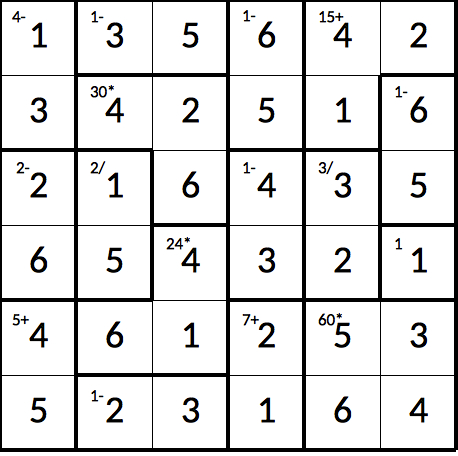
\includegraphics[scale=0.333]{Gambar/hybridgenetic/Generation1Chromosome1}
\caption[Kromosom 1 dalam Generasi ke-1]{Kromosom 1 dalam Generasi ke-1}
\label{fig:analisisg1k1}
\end{figure}

\begin{figure}
\centering
\captionsetup{justification=centering}
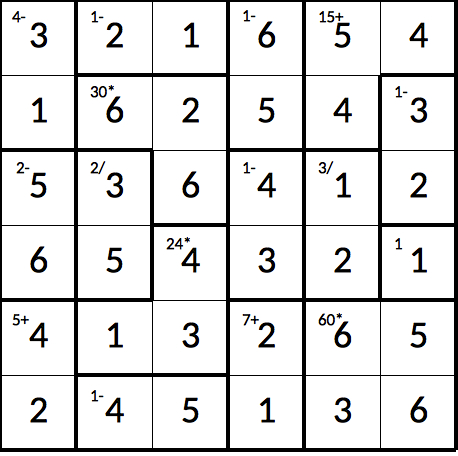
\includegraphics[scale=0.333]{Gambar/hybridgenetic/Generation1Chromosome2}
\caption[Kromosom 2 dalam Generasi ke-1]{Kromosom 2 dalam Generasi ke-1}
\label{fig:analisisg1k2}
\end{figure}

\begin{figure}
\centering
\captionsetup{justification=centering}
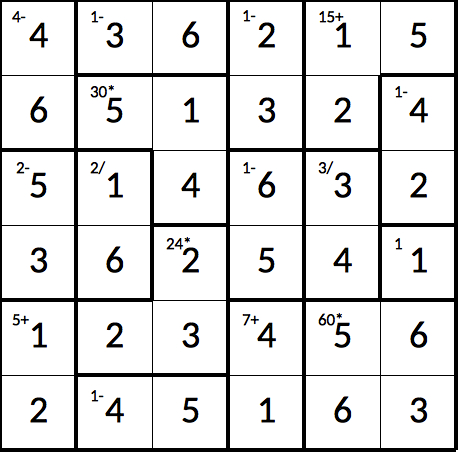
\includegraphics[scale=0.333]{Gambar/hybridgenetic/Generation1Chromosome3}
\caption[Kromosom 3 dalam Generasi ke-1]{Kromosom 3 dalam Generasi ke-1}
\label{fig:analisisg1k3}
\end{figure}

\begin{figure}
\centering
\captionsetup{justification=centering}
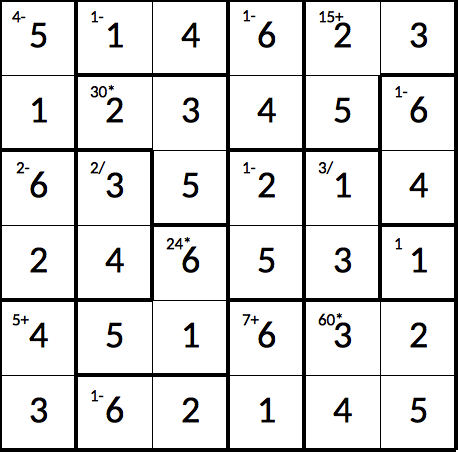
\includegraphics[scale=0.333]{Gambar/hybridgenetic/Generation1Chromosome4}
\caption[Kromosom 4 dalam Generasi ke-1]{Kromosom 4 dalam Generasi ke-1}
\label{fig:analisisg1k4}
\end{figure}

\begin{figure}
\centering
\captionsetup{justification=centering}
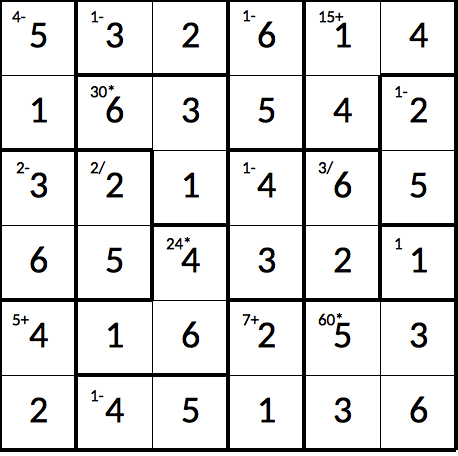
\includegraphics[scale=0.333]{Gambar/hybridgenetic/Generation1Chromosome5}
\caption[Kromosom 5 dalam Generasi ke-1]{Kromosom 5 dalam Generasi ke-1}
\label{fig:analisisg1k5}
\end{figure}

\begin{figure}
\centering
\captionsetup{justification=centering}
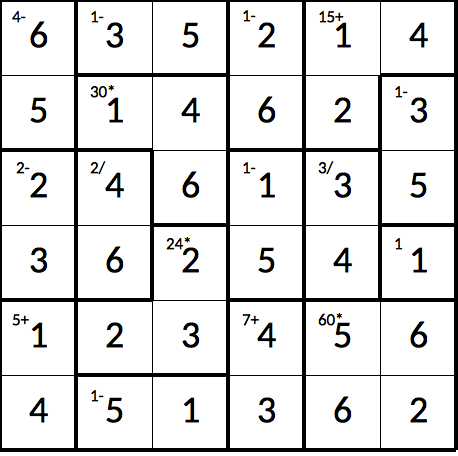
\includegraphics[scale=0.333]{Gambar/hybridgenetic/Generation1Chromosome6}
\caption[Kromosom 6 dalam Generasi ke-1]{Kromosom 6 dalam Generasi ke-1}
\label{fig:analisisg1k6}
\end{figure}

\begin{figure}
\centering
\captionsetup{justification=centering}
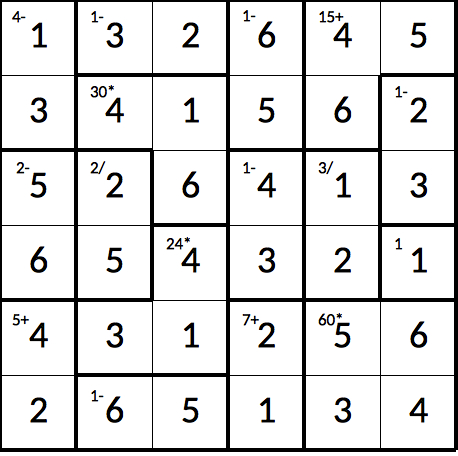
\includegraphics[scale=0.333]{Gambar/hybridgenetic/Generation1Chromosome7}
\caption[Kromosom 7 dalam Generasi ke-1]{Kromosom 7 dalam Generasi ke-1}
\label{fig:analisisg1k7}
\end{figure}

\begin{figure}
\centering
\captionsetup{justification=centering}
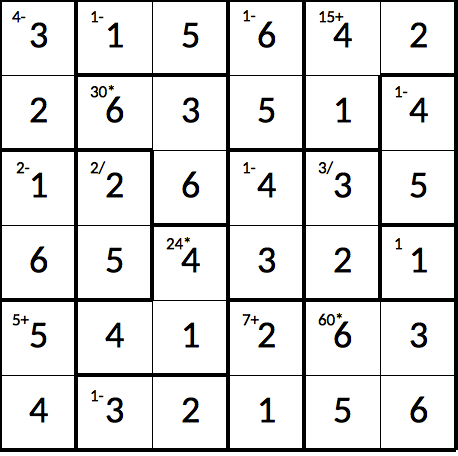
\includegraphics[scale=0.333]{Gambar/hybridgenetic/Generation1Chromosome8}
\caption[Kromosom 8 dalam Generasi ke-1]{Kromosom 8 dalam Generasi ke-1}
\label{fig:analisisg1k8}
\end{figure}

\begin{figure}
\centering
\captionsetup{justification=centering}
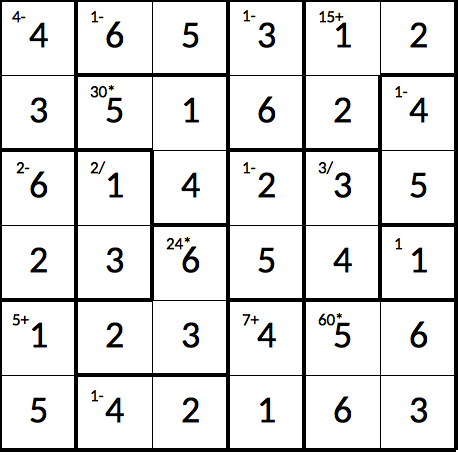
\includegraphics[scale=0.333]{Gambar/hybridgenetic/Generation1Chromosome9}
\caption[Kromosom 9 dalam Generasi ke-1]{Kromosom 9 dalam Generasi ke-1}
\label{fig:analisisg1k9}
\end{figure}

\begin{figure}
\centering
\captionsetup{justification=centering}
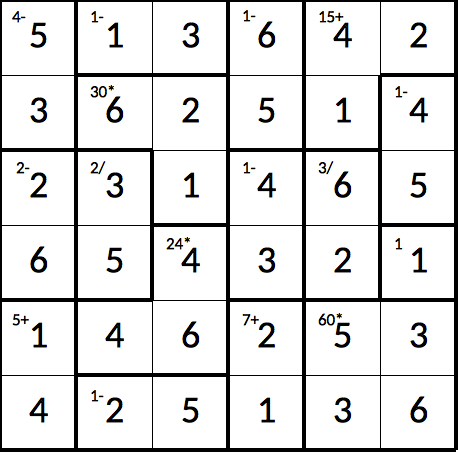
\includegraphics[scale=0.333]{Gambar/hybridgenetic/Generation1Chromosome10}
\caption[Kromosom 10 dalam Generasi ke-1]{Kromosom 10 dalam Generasi ke-1}
\label{fig:analisisg1k10}
\end{figure}

\begin{figure}
\centering
\captionsetup{justification=centering}
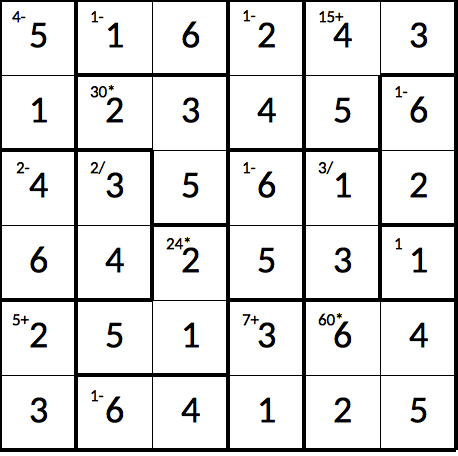
\includegraphics[scale=0.333]{Gambar/hybridgenetic/Generation1Chromosome11}
\caption[Kromosom 11 dalam Generasi ke-1]{Kromosom 11 dalam Generasi ke-1}
\label{fig:analisisg1k11}
\end{figure}

\begin{figure}
\centering
\captionsetup{justification=centering}
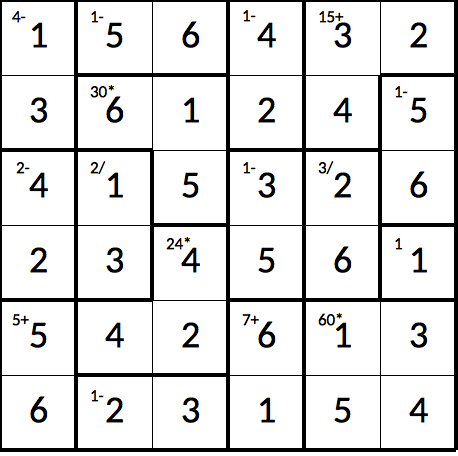
\includegraphics[scale=0.333]{Gambar/hybridgenetic/Generation1Chromosome12}
\caption[Kromosom 12 dalam Generasi ke-1]{Kromosom 12 dalam Generasi ke-1}
\label{fig:analisisg1k12}
\end{figure}

\clearpage

Berdasarkan nilai kelayakan untuk kromosom-kromosom pada Generasi ke-1 yang ditampilkan pada Tabel~\ref{tab:analisishg2}, 5 kromosom terbaik akan diambil untuk menjadi bagian dari Generasi ke-2. Ke-5 kromosom yang terpilih adalah Kromosom 12, Kromosom 5, Kromosom 7, Kromosom 11, dan Kromosom 1.

\begin{table}
\centering
\captionsetup{justification=centering}
\caption[Tabel nilai kelayakan untuk kromosom-kromsom pada Generasi ke-1]{Tabel nilai kelayakan untuk kromosom-kromsom pada Generasi ke-1}
\begin{tabular}{| l | l |}
\hline
Nomor Kromosom & Nilai Kelayakan \\
\hline \hline
1 & 0,3333 \\
\hline
2 & 0,3056 \\
\hline
3 & 0,25 \\
\hline
4 & 0,2222 \\
\hline
5 & 0,4444 \\
\hline
6 & 0,1389 \\
\hline
7 & 0,3889 \\
\hline
8 & 0,25 \\
\hline
9 & 0,1389 \\
\hline
10 & 0,3056 \\
\hline
11 & 0,3889 \\
\hline
12 & 0,5556 \\
\hline
\end{tabular}
\label{tab:analisishg2}
\end{table}

Untuk Generasi ke-2, 5 kromosom adalah 5 kromosom terbaik dari Generasi ke-1, 6 kromosom adalah hasil kawin silang dari 2 kromosom dari Generasi ke-1, dan 1 kromosom adalah hasil mutasi dari 1 kromosom dari Generasi ke-1.

Gambar~\ref{fig:analisisg2k1} menggambarkan Kromosom 1, yaitu Kromosom 12 dari Generasi ke-1, gambar~\ref{fig:analisisg2k2} menggambarkan Kromosom 2, yaitu Kromosom 5 dari Generasi ke-1, gambar~\ref{fig:analisisg2k3} menggambarkan Kromosom 3, yaitu Kromosom 7 dari Generasi ke-1, gambar~\ref{fig:analisisg2k4} menggambarkan Kromosom 4, yaitu Kromosom 11 dari Generasi ke-1, gambar~\ref{fig:analisisg2k5} menggambarkan Kromosom 5, yaitu Kromosom 1 dari Generasi ke-1, gambar~\ref{fig:analisisg2k6} menggambarkan Kromosom 6, yaitu hasil kawin silang dari Kromosom 5 dan Kromosom 12 dari Generasi ke-1, gambar~\ref{fig:analisisg2k7} menggambarkan Kromosom 7, yaitu hasil kawin silang dari Kromosom 3 dan Kromosom 8 dari Generasi ke-1, gambar~\ref{fig:analisisg2k8} menggambarkan Kromosom 8, yaitu hasil kawin silang dari Kromosom 7 dan Kromosom 10 dari Generasi ke-1, gambar~\ref{fig:analisisg2k9} menggambarkan Kromosom 9, yaitu hasil kawin silang dari Kromosom 7 dan Kromosom 10 dari Generasi ke-1, gambar~\ref{fig:analisisg2k10} menggambarkan Kromosom 10, yaitu hasil kawin silang dari Kromosom 2 dan Kromosom 5 dari Generasi ke-1, gambar~\ref{fig:analisisg2k11} menggambarkan Kromosom 11, yaitu hasil kawin silang dari Kromosom 2 dan Kromosom 5 dari Generasi ke-1, dan gambar~\ref{fig:analisisg2k12} menggambarkan Kromosom 12, yaitu hasil mutasi dari Kromosom 12 dari Generasi ke-1.

\clearpage

\begin{figure}
\centering
\captionsetup{justification=centering}
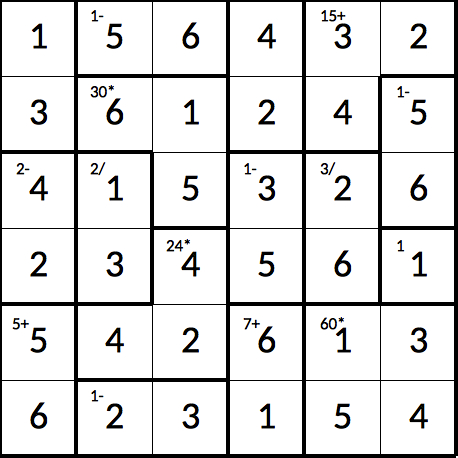
\includegraphics[scale=0.333]{Gambar/hybridgenetic/Generation2Chromosome1}
\caption[Kromosom 1 dalam Generasi ke-2]{Kromosom 1 dalam Generasi ke-2}
\label{fig:analisisg2k1}
\end{figure}

\begin{figure}
\centering
\captionsetup{justification=centering}
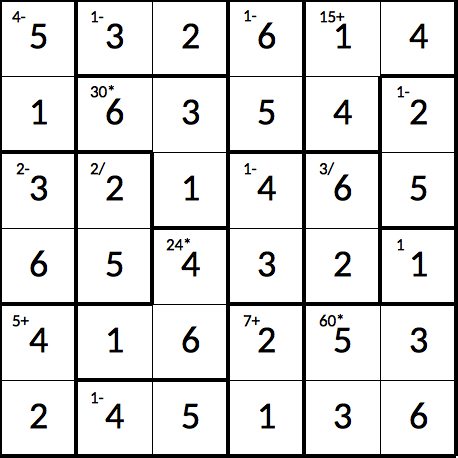
\includegraphics[scale=0.333]{Gambar/hybridgenetic/Generation2Chromosome2}
\caption[Kromosom 2 dalam Generasi ke-2]{Kromosom 2 dalam Generasi ke-2}
\label{fig:analisisg2k2}
\end{figure}

\begin{figure}
\centering
\captionsetup{justification=centering}
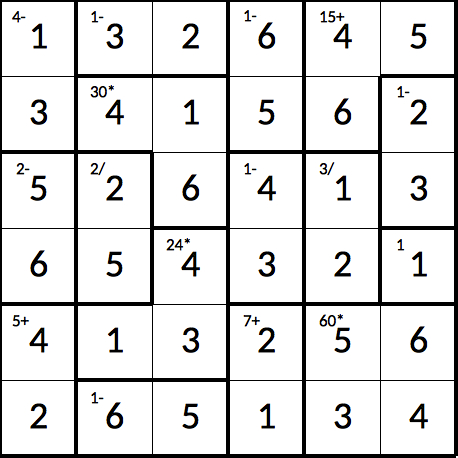
\includegraphics[scale=0.333]{Gambar/hybridgenetic/Generation2Chromosome3}
\caption[Kromosom 3 dalam Generasi ke-2]{Kromosom 3 dalam Generasi ke-2}
\label{fig:analisisg2k3}
\end{figure}

\begin{figure}
\centering
\captionsetup{justification=centering}
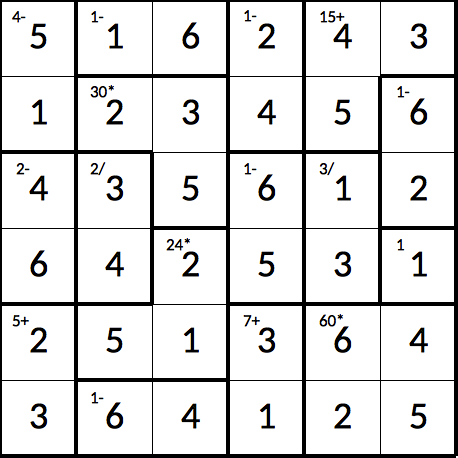
\includegraphics[scale=0.333]{Gambar/hybridgenetic/Generation2Chromosome4}
\caption[Kromosom 4 dalam Generasi ke-2]{Kromosom 4 dalam Generasi ke-2}
\label{fig:analisisg2k4}
\end{figure}

\begin{figure}
\centering
\captionsetup{justification=centering}
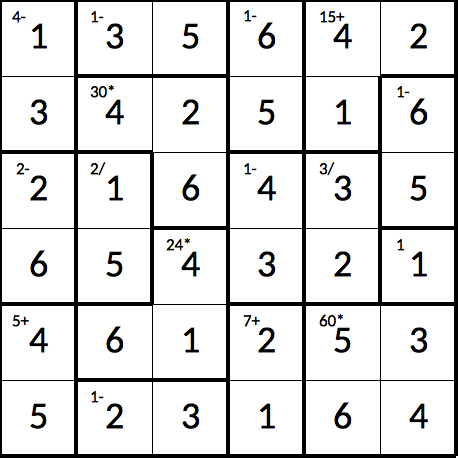
\includegraphics[scale=0.333]{Gambar/hybridgenetic/Generation2Chromosome5}
\caption[Kromosom 5 dalam Generasi ke-2]{Kromosom 5 dalam Generasi ke-2}
\label{fig:analisisg2k5}
\end{figure}

\begin{figure}
\centering
\captionsetup{justification=centering}
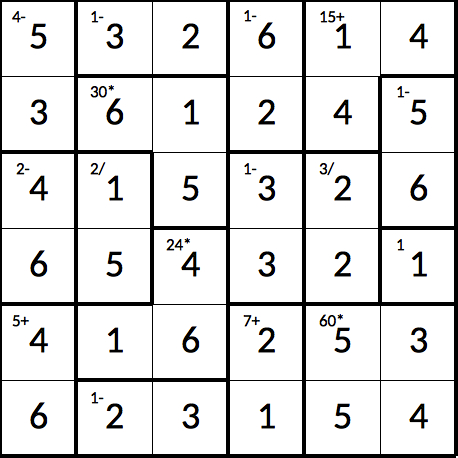
\includegraphics[scale=0.333]{Gambar/hybridgenetic/Generation2Chromosome6}
\caption[Kromosom 6 dalam Generasi ke-2]{Kromosom 6 dalam Generasi ke-2}
\label{fig:analisisg2k6}
\end{figure}

\begin{figure}
\centering
\captionsetup{justification=centering}
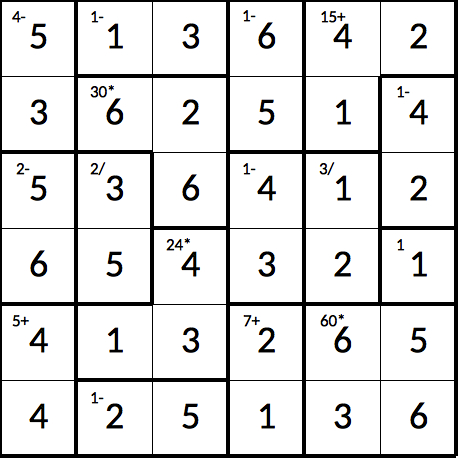
\includegraphics[scale=0.333]{Gambar/hybridgenetic/Generation2Chromosome7}
\caption[Kromosom 7 dalam Generasi ke-2]{Kromosom 7 dalam Generasi ke-2}
\label{fig:analisisg2k7}
\end{figure}

\begin{figure}
\centering
\captionsetup{justification=centering}
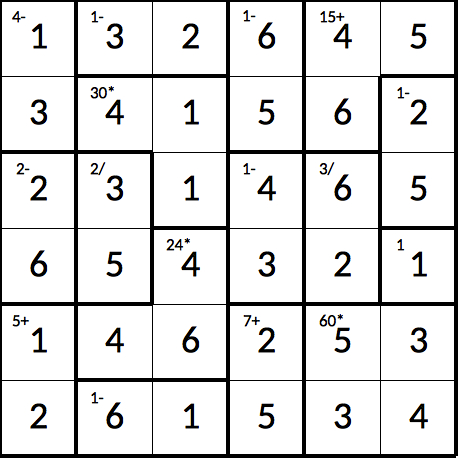
\includegraphics[scale=0.333]{Gambar/hybridgenetic/Generation2Chromosome8}
\caption[Kromosom 8 dalam Generasi ke-2]{Kromosom 8 dalam Generasi ke-2}
\label{fig:analisisg2k8}
\end{figure}

\begin{figure}
\centering
\captionsetup{justification=centering}
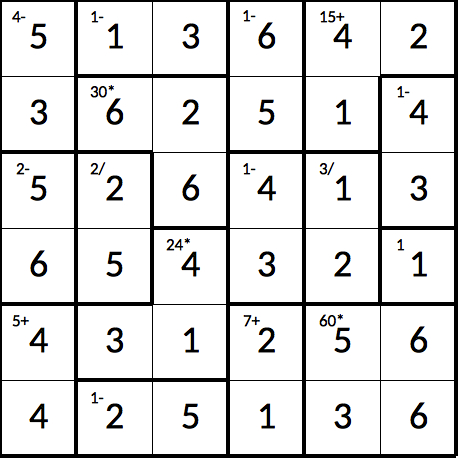
\includegraphics[scale=0.333]{Gambar/hybridgenetic/Generation2Chromosome9}
\caption[Kromosom 9 dalam Generasi ke-2]{Kromosom 9 dalam Generasi ke-2}
\label{fig:analisisg2k9}
\end{figure}

\begin{figure}
\centering
\captionsetup{justification=centering}
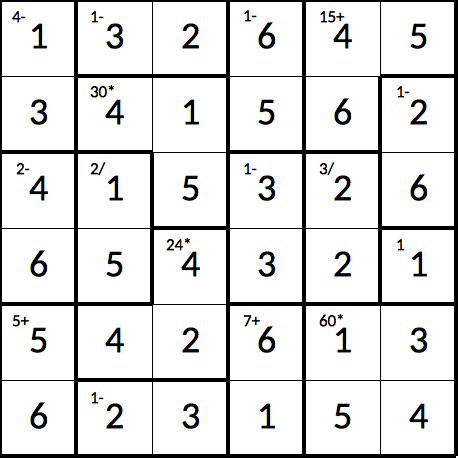
\includegraphics[scale=0.333]{Gambar/hybridgenetic/Generation2Chromosome10}
\caption[Kromosom 10 dalam Generasi ke-2]{Kromosom 10 dalam Generasi ke-2}
\label{fig:analisisg2k10}
\end{figure}

\begin{figure}
\centering
\captionsetup{justification=centering}
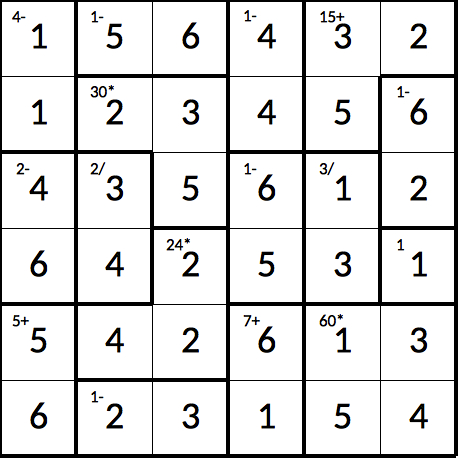
\includegraphics[scale=0.333]{Gambar/hybridgenetic/Generation2Chromosome11}
\caption[Kromosom 11 dalam Generasi ke-2]{Kromosom 11 dalam Generasi ke-2}
\label{fig:analisisg2k11}
\end{figure}

\begin{figure}
\centering
\captionsetup{justification=centering}
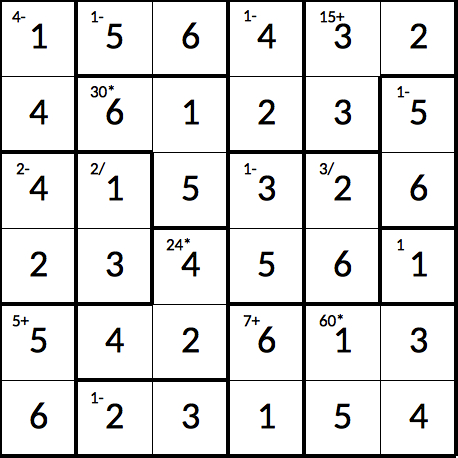
\includegraphics[scale=0.333]{Gambar/hybridgenetic/Generation2Chromosome12}
\caption[Kromosom 12 dalam Generasi ke-2]{Kromosom 12 dalam Generasi ke-2}
\label{fig:analisisg2k12}
\end{figure}

\clearpage

Berdasarkan nilai kelayakan untuk kromosom-kromosom pada Generasi ke-2 yang ditampilkan pada Tabel~\ref{tab:analisishg3}, 5 kromosom terbaik akan diambil untuk menjadi bagian dari Generasi ke-3. Ke-5 kromosom yang terpilih adalah Kromosom 1, Kromosom 12, Kromosom 2, Kromosom 3, dan Kromosom 4.

\begin{table}
\centering
\captionsetup{justification=centering}
\caption[Tabel nilai kelayakan untuk kromosom-kromsom pada Generasi ke-1]{Tabel nilai kelayakan untuk kromosom-kromsom pada Generasi ke-2}
\begin{tabular}{| l | l |}
\hline
Nomor Kromosom & Nilai Kelayakan \\
\hline \hline
1 & 0,5556 \\
\hline
2 & 0,4444 \\
\hline
3 & 0,3889 \\
\hline
4 & 0,3889 \\
\hline
5 & 0,3333 \\
\hline
6 & 0,1944 \\
\hline
7 & 0,1389 \\
\hline
8 & 0,0833 \\
\hline
9 & 0,25 \\
\hline
10 & 0,1944 \\
\hline
11 & 0,1944 \\
\hline
12 & 0,5 \\
\hline
\end{tabular}
\label{tab:analisishg3}
\end{table}

Untuk Generasi ke-3, 5 kromosom adalah 5 kromosom terbaik dari Generasi ke-2, 6 kromosom adalah hasil kawin silang dari 2 kromosom dari Generasi ke-2, dan 1 kromosom adalah hasil mutasi dari 1 kromosom dari Generasi ke-2.

Gambar~\ref{fig:analisisg3k1} menggambarkan Kromosom 1, yaitu Kromosom 1 dari Generasi ke-2, Gambar~\ref{fig:analisisg3k2} menggambarkan Kromosom 2, yaitu Kromosom 12 dari Generasi ke-2, Gambar~\ref{fig:analisisg3k3} menggambarkan Kromosom 3, yaitu Kromosom 2 dari Generasi ke-2, Gambar~\ref{fig:analisisg3k4} menggambarkan Kromosom 4, yaitu Kromosom 3 dari Generasi ke-2, Gambar~\ref{fig:analisisg3k5} menggambarkan Kromosom 5, yaitu Kromosom 4 dari Generasi ke-2, Gambar~\ref{fig:analisisg3k6} menggambarkan Kromosom 6, yaitu hasil kawin silang dari Kromosom 2 dan Kromosom 12 dari Generasi ke-2, Gambar~\ref{fig:analisisg3k7} menggambarkan Kromosom 7, yaitu hasil kawin silang dari Kromosom 2 dan Kromosom 12 dari Generasi ke-2, Gambar~\ref{fig:analisisg3k8} menggambarkan Kromosom 8, yaitu hasil kawin silang dari Kromosom 5 dan Kromosom 9 dari Generasi ke-2, Gambar~\ref{fig:analisisg3k9} menggambarkan Kromosom 9, yaitu hasil kawin silang dari Kromosom 5 dan Kromosom 9 dari Generasi ke-2, Gambar~\ref{fig:analisisg3k10} menggambarkan Kromosom 10, yaitu hasil kawin silang dari Kromosom 5 dan Kromosom 6 dari Generasi ke-2, Gambar~\ref{fig:analisisg3k11} menggambarkan Kromosom 11, yaitu hasil kawin silang dari Kromosom 5 dan Kromosom 6 dari Generasi ke-2, dan Gambar~\ref{fig:analisisg3k12} menggambarkan Kromosom 12, yaitu hasil mutasi dari Kromosom 2 dari Generasi ke-2.

\clearpage

\begin{figure}
\centering
\captionsetup{justification=centering}
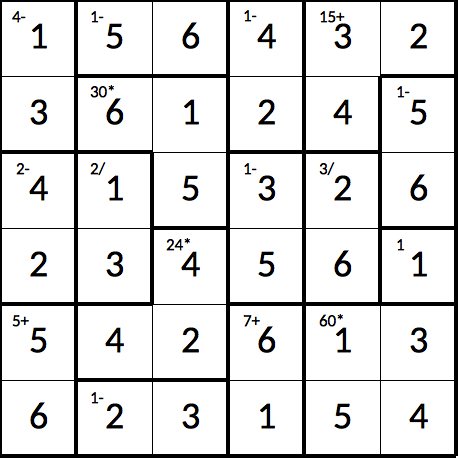
\includegraphics[scale=0.333]{Gambar/hybridgenetic/Generation3Chromosome1}
\caption[Kromosom 1 dalam Generasi ke-3]{Kromosom 1 dalam Generasi ke-3}
\label{fig:analisisg3k1}
\end{figure}

\begin{figure}
\centering
\captionsetup{justification=centering}
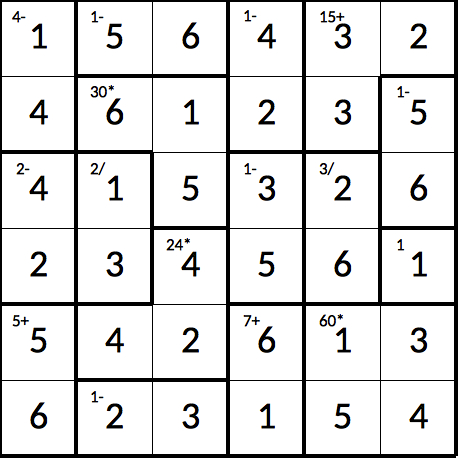
\includegraphics[scale=0.333]{Gambar/hybridgenetic/Generation3Chromosome2}
\caption[Kromosom 2 dalam Generasi ke-3]{Kromosom 2 dalam Generasi ke-3}
\label{fig:analisisg3k2}
\end{figure}

\begin{figure}
\centering
\captionsetup{justification=centering}
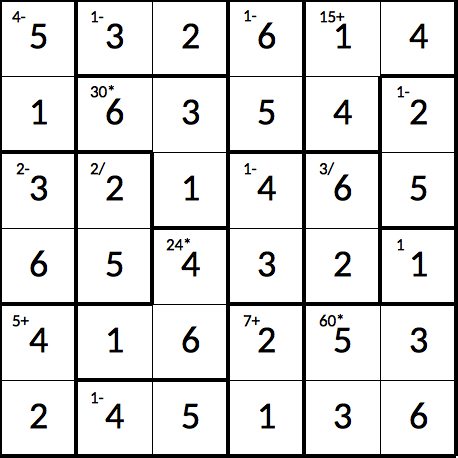
\includegraphics[scale=0.333]{Gambar/hybridgenetic/Generation3Chromosome3}
\caption[Kromosom 3 dalam Generasi ke-3]{Kromosom 3 dalam Generasi ke-3}
\label{fig:analisisg3k3}
\end{figure}

\begin{figure}
\centering
\captionsetup{justification=centering}
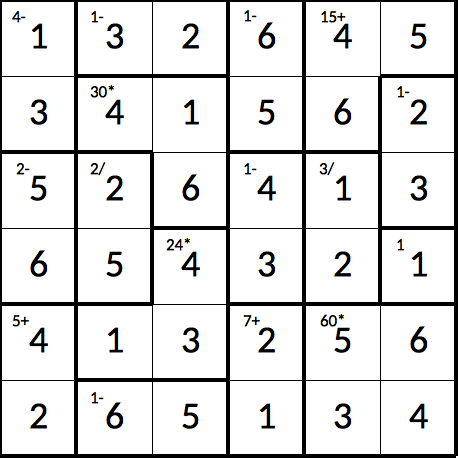
\includegraphics[scale=0.333]{Gambar/hybridgenetic/Generation3Chromosome4}
\caption[Kromosom 4 dalam Generasi ke-3]{Kromosom 4 dalam Generasi ke-3}
\label{fig:analisisg3k4}
\end{figure}

\begin{figure}
\centering
\captionsetup{justification=centering}
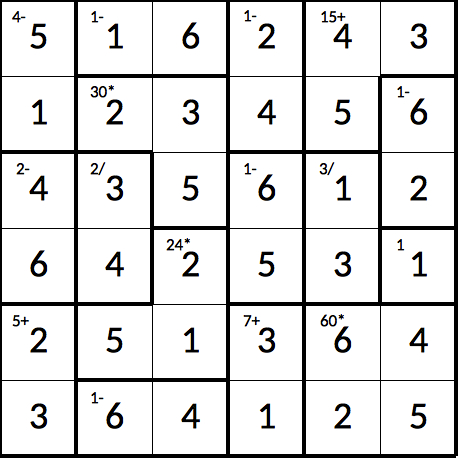
\includegraphics[scale=0.333]{Gambar/hybridgenetic/Generation3Chromosome5}
\caption[Kromosom 5 dalam Generasi ke-3]{Kromosom 5 dalam Generasi ke-3}
\label{fig:analisisg3k5}
\end{figure}

\begin{figure}
\centering
\captionsetup{justification=centering}
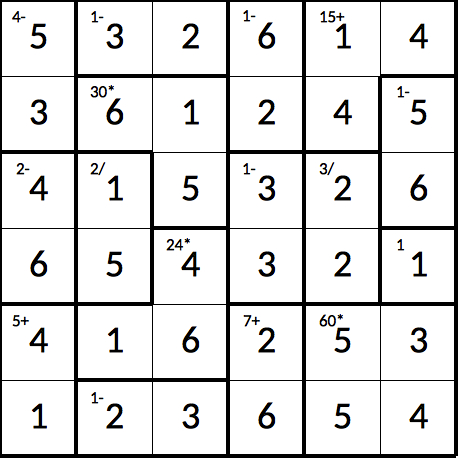
\includegraphics[scale=0.333]{Gambar/hybridgenetic/Generation3Chromosome6}
\caption[Kromosom 6 dalam Generasi ke-3]{Kromosom 6 dalam Generasi ke-3}
\label{fig:analisisg3k6}
\end{figure}

\begin{figure}
\centering
\captionsetup{justification=centering}
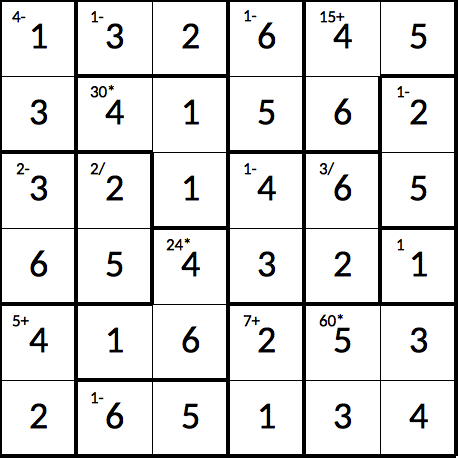
\includegraphics[scale=0.333]{Gambar/hybridgenetic/Generation3Chromosome7}
\caption[Kromosom 7 dalam Generasi ke-3]{Kromosom 7 dalam Generasi ke-3}
\label{fig:analisisg3k7}
\end{figure}

\begin{figure}
\centering
\captionsetup{justification=centering}
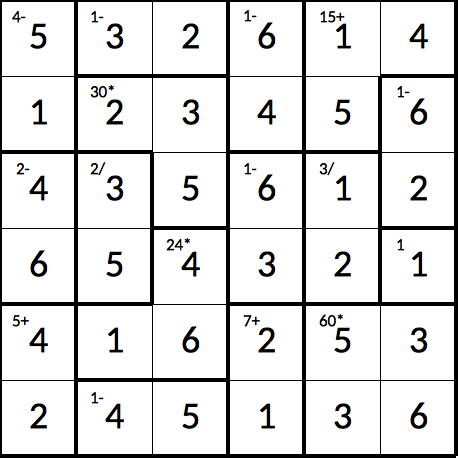
\includegraphics[scale=0.333]{Gambar/hybridgenetic/Generation3Chromosome8}
\caption[Kromosom 8 dalam Generasi ke-3]{Kromosom 8 dalam Generasi ke-3}
\label{fig:analisisg3k8}
\end{figure}

\begin{figure}
\centering
\captionsetup{justification=centering}
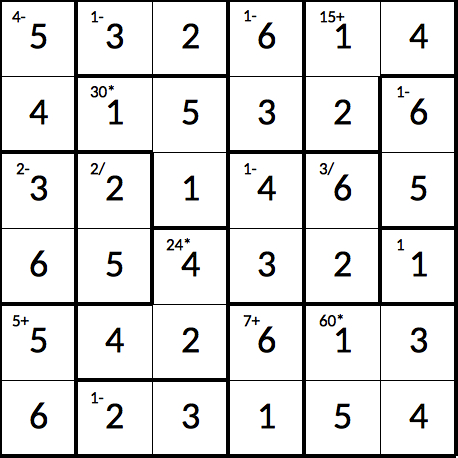
\includegraphics[scale=0.333]{Gambar/hybridgenetic/Generation3Chromosome9}
\caption[Kromosom 9 dalam Generasi ke-3]{Kromosom 9 dalam Generasi ke-3}
\label{fig:analisisg3k9}
\end{figure}

\begin{figure}
\centering
\captionsetup{justification=centering}
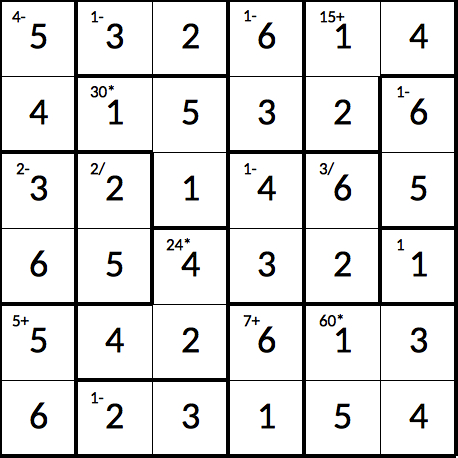
\includegraphics[scale=0.333]{Gambar/hybridgenetic/Generation3Chromosome10}
\caption[Kromosom 10 dalam Generasi ke-3]{Kromosom 10 dalam Generasi ke-3}
\label{fig:analisisg3k10}
\end{figure}

\begin{figure}
\centering
\captionsetup{justification=centering}
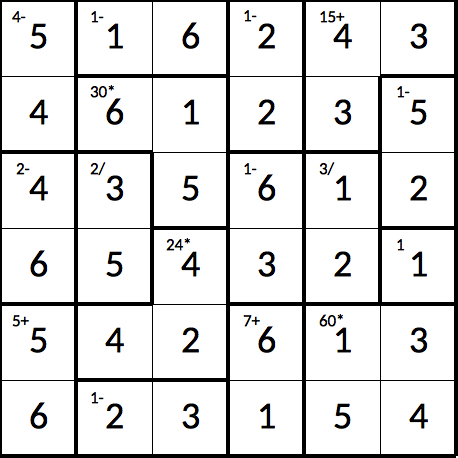
\includegraphics[scale=0.333]{Gambar/hybridgenetic/Generation3Chromosome11}
\caption[Kromosom 11 dalam Generasi ke-3]{Kromosom 11 dalam Generasi ke-3}
\label{fig:analisisg3k11}
\end{figure}

\begin{figure}
\centering
\captionsetup{justification=centering}
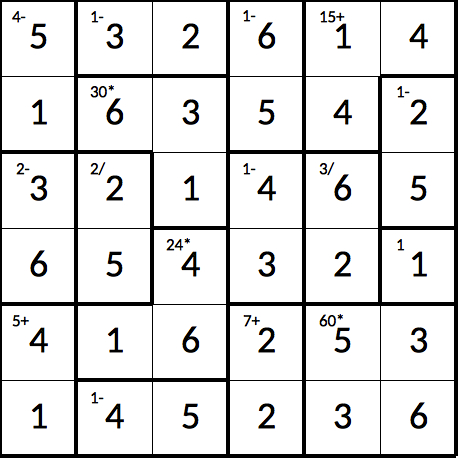
\includegraphics[scale=0.333]{Gambar/hybridgenetic/Generation3Chromosome12}
\caption[Kromosom 12 dalam Generasi ke-3]{Kromosom 12 dalam Generasi ke-3}
\label{fig:analisisg3k12}
\end{figure}

\clearpage

Berdasarkan nilai kelayakan untuk kromosom-kromosom pada Generasi ke-3 yang ditampilkan pada Tabel~\ref{tab:analisishg4}, 5 kromosom terbaik akan diambil untuk menjadi bagian dari Generasi ke-4. Ke-5 kromosom yang terpilih adalah Kromosom 1, Kromosom 2, Kromosom 3, Kromosom 4, dan Kromosom 12.

\begin{table}
\centering
\captionsetup{justification=centering}
\caption[Tabel nilai kelayakan untuk kromosom-kromsom pada Generasi ke-3]{Tabel nilai kelayakan untuk kromosom-kromsom pada Generasi ke-3}
\begin{tabular}{| l | l |}
\hline
Nomor Kromosom & Nilai Kelayakan \\
\hline \hline
1 & 0,5556 \\
\hline
2 & 0,5 \\
\hline
3 & 0,4444 \\
\hline
4 & 0,3889 \\
\hline
5 & 0,3889 \\
\hline
6 & 0,2778 \\
\hline
7 & 0,1389 \\
\hline
8 & 0,1389 \\
\hline
9 & 0,1389 \\
\hline
10 & 0,1389 \\
\hline
11 & 0,1944 \\
\hline
12 & 0,3889 \\
\hline
\end{tabular}
\label{tab:analisishg4}
\end{table}

Proses ini diulang untuk menghasilkan generasi-generasi berikutnya, sampai algoritma genetik dapat menemukan solusi dari teka-teki Calcudoku tersebut.

\section{Perangkat Lunak}
\label{sec:analisispl}

Berdasarkan landasan teori dan analisis algoritma \textit{backtracking} dan \textit{hybrid genetic} untuk menyelesaikan permainan teka-teki Calcudoku yang telah dilakukan, perangkat lunak Calcudoku akan dibuat. Perangkat lunak ini akan menerima masukan dalam bentuk \textit{file} yang berisi:

\begin{enumerate}
\item Ukuran \textit{grid}.
\item Jumlah \textit{cage}.
\item Matriks \textit{cage assignment}, yang merepresentasikan posisi dari setiap \textit{cage} dalam \textit{grid}.
\item Matriks \textit{cage objectives}, yang berisikan angka tujuan dan operasi matematika yang telah ditentukan untuk setiap \textit{cage}.
\end{enumerate}

Perangkat lunak ini akan menghasilkan keluaran berupa antarmuka grafis permainan teka-teki Calcudoku berdasarkan isi \textit{file}  yang di-\textit{load} oleh pengguna. Permainan ini dapat diselesaikan oleh pengguna dengan usahanya sendiri, atau menggunakan salah satu dari dua \textit{solver} yang disediakan.  Kedua \textit{solver} tersebut yaitu:

\begin{enumerate}
\item Algoritma \textit{backtracking}, dan
\item Algoritma \textit{hybrid genetic}.
\end{enumerate}

Pengguna dapat me-\textit{load} file masukan untuk memulai permainan, me-\textit{reset} permainan untuk mengulang permainan berdasarkan \textit{file} masukan yang sudah di-\textit{load} dari awal, dan menutup \textit{file} masukan untuk mengakhiri permainan, atau jika ingin me-\textit{load file} masukan yang lain. Pengguna juga dapat meminta perangkat lunak untuk memeriksa permainan jika ada masukan yang salah di dalam \textit{grid}, misalnya ada angka yang berulang dalam sebuah baris atau kolom, atau angka-angka dalam sebuah \textit{cage} tidak mencapai angka tujuan yang ditentukan setelah dihitung dengan operasi matematika yang ditentukan. Pemain juga dapat mengatur nilai dari parameter-parameter untuk algoritma genetik.

Kebutuhan-kebutuhan yang diperlukan oleh perangkat lunak ini akan dijelaskan menggunakan diagram \textit{use cage}, dan skenario.

\subsection{Diagram \textit{Use Case} dan Skenario}
\label{sec:analisisusecase}

Diagram \textit{use case} adalah diagram yang menggambarkan interaksi antara sistem (perangkat lunak) dengan pengguna. Berdasarkan analisis perangkat lunak yang telah dilakukan, maka pengguna dapat:

\begin{enumerate}
\item Membuka file masukan untuk memulai permainan.
\item Memilih salah satu dari dua \textit{solver} yang disediakan untuk menyelesaikan permainan berdasarkan \textit{file} yang sudah di-\textit{load}.
\item Me-\textit{reset} permainan untuk mengulang permainan berdasarkan \textit{file} masukan yang sudah di-\textit{load} dari awal.
\item Meminta perangkat lunak untuk memeriksa permainan jika ada masukan yang salah di dalam \textit{grid}.
\item Menutup \textit{file} masukan untuk mengakhiri permainan.
\item Menyelesaikan permainan dengan usahanya sendiri.
\item Mengatur nilai dari parameter-parameter untuk algoritma genetik.
\end{enumerate}

Diagram \textit{use case} untuk perangkat lunak permainan teka-teki Calcudoku dapat dilihat pada Gambar~\ref{fig:analisisusecase}.

\begin{figure}
\centering
\captionsetup{justification=centering}
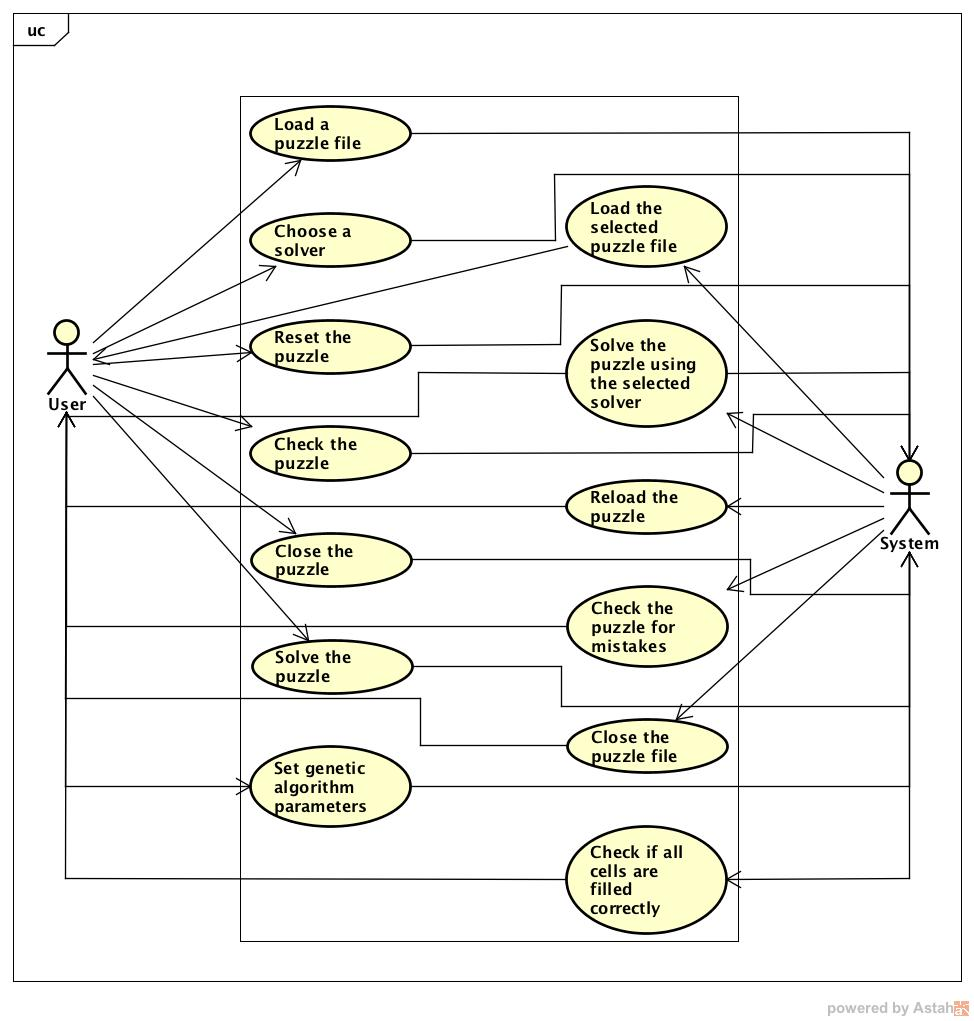
\includegraphics[scale=0.4]{Gambar/Analisis/DiagramUseCase}
\caption[Diagram \textit{use case} untuk perangkat lunak permainan teka-teki Calcudoku]{Diagram \textit{use case} untuk perangkat lunak permainan teka-teki Calcudoku}
\label{fig:analisisusecase}
\end{figure}

Berdasarkan diagram \textit{use case} yang dapat dilihat pada Gambar~\ref{fig:analisisusecase}, skenario-skenario yang dapat dilakukan oleh pengguna adalah:

\begin{enumerate}
\item Membuka {file} masukan. Penjelasan untuk skenario ini dapat dilihat pada Tabel~\ref{tab:analisisload}.

\begin{table}
\centering
\captionsetup{justification=centering}
\caption[Skenario me-\textit{load file}]{Skenario me-\textit{load file}}
\begin{tabular}{| l || l |}
\hline
Nama & Membuka {file} masukan \\
\hline
Aktor & Pengguna \\
\hline
Deskripsi & Memembuka file masukan untuk memulai permainan. \\
\hline
Kondisi Awal & Perangkat lunak belum membuka {file} masukan. \\
\hline
Kondisi Akhir & Perangkat lunak sudah membuka {file} masukan .\\
\hline
Skenario Utama & \makecell[l]{Pengguna masuk ke dalam menu "\textit{File}", lalu memilih menu \textit{item} "\textit{Load} \\ \textit{Puzzle File}", lalu memilih \textit{file} masukan yang akan dibuka, dan mengklik \\ tombol "OK". Jika perangkat lunak sudah membuka {file} masukan, dan ingin \\ membuka {file} masukan yang baru, akan keluar kotak dialog "\textit{Are you sure} \\  \textit{you want to load another puzzle file}?", klik tombol "\textit{Yes}" untuk membuka {file} \\ masukan baru, atau klik tombol "\textit{No}" untuk membatalkan.} \\
\hline
\end{tabular}
\label{tab:analisisload}
\end{table}

\item Memilih salah satu dari dua \textit{solver} yang disediakan. Penjelasan untuk skenario ini dapat dilihat pada Tabel~\ref{tab:analisischoose}

\begin{table}
\centering
\captionsetup{justification=centering}
\caption[Skenario memilih salah satu dari dua \textit{solver} yang disediakan]{Skenario memilih salah satu dari dua \textit{solver} yang disediakan}
\begin{tabular}{| l || l |}
\hline
Nama & Memilih salah satu dari dua \textit{solver} yang disediakan \\
\hline
Aktor & Pengguna \\
\hline
Deskripsi & \makecell[l]{Memilih salah satu dari dua \textit{solver} yang disediakan untuk menyelesaikan \\ permainan berdasarkan \textit{file} yang sudah di-\textit{load}.} \\
\hline
Kondisi Awal & \textit{Solver} belum menyelesaikan permainan. \\
\hline
Kondisi Akhir & \textit{Solver} berhasil atau gagal dalam menyelesaikan permainan. \\
\hline
Skenario Utama & \makecell[l]{Pengguna masuk ke dalam menu "\textit{Solve}", lalu memilih salah satu dari dua \\\textit{solver} yang disediakan. Pemain memilih menu \textit{item} "\textit{Backtracking}" untuk \\ memilih \textit{solver} dengan algoritma \textit{backtracking}, atau menu \textit{item} "\textit{Hybrid} \\ \textit{Genetic}" untuk memilih \textit{solver} dengan algoritma \textit{hybrid genetic}.} \\
\hline
\end{tabular}
\label{tab:analisischoose}
\end{table}

\item Me-\textit{reset} permainan. Penjelasan untuk skenario ini dapat dilihat pada Tabel~\ref{tab:analisisreset}.

\begin{table}
\centering
\captionsetup{justification=centering}
\caption[Skenario me-\textit{reset} permainan]{Skenario me-\textit{reset} permainan}
\begin{tabular}{| l || l |}
\hline
Nama & Me-\textit{reset} permainan \\
\hline
Aktor & Pengguna \\
\hline
Deskripsi & \makecell[l]{Me-\textit{reset} permainan untuk mengulang permainan berdasarkan \textit{file} masukan \\ yang sudah di-\textit{load} dari awal.} \\
\hline
Kondisi Awal & \makecell[l]{Permainan belum di-\textit{reset}, sel-sel dalam \textit{grid} mungkin masih berisi angka- \\ angka.} \\
\hline
Kondisi Akhir & \makecell[l]{Permainan sudah di-\textit{reset}, semua sel-sel dalam \textit{grid} sudah dalam keadaan \\ kosong.} \\
\hline
Skenario Utama & \makecell[l]{Pengguna masuk ke dalam menu "\textit{File}", lalu memilih menu \textit{item} "\textit{Reset} \\ \textit{Puzzle File}". Akan keluar kotak dialog "\textit{Are you sure you want to reset this} \\ \textit{puzzle?}", klik tombol "\textit{Yes} untuk me-\textit{reset} permainan, atau klik tombol \\ "\textit{No}" untuk membatalkan. Jika perangkat lunak belum me-\textit{load file} \\ masukan, maka akan keluar pesan \textit{error} "\textit{Puzzle file not loaded}".} \\
\hline
\end{tabular}
\label{tab:analisisreset}
\end{table}

\item Meminta perangkat lunak untuk memeriksa permainan. Penjelasan untuk skenario ini dapat dilihat pada Tabel~\ref{tab:analisischeck}.

\begin{table}
\centering
\captionsetup{justification=centering}
\caption[Skenario meminta perangkat lunak untuk memeriksa permainan]{Skenario meminta perangkat lunak untuk memeriksa permainan}
\begin{tabular}{| l || l |}
\hline
Nama & Meminta perangkat lunak untuk memeriksa permainan \\
\hline
Aktor & Pengguna \\
\hline
Deskripsi & \makecell[l]{Meminta perangkat lunak untuk memeriksa permainan jika ada masukan \\ yang salah di dalam \textit{grid}.} \\
\hline
Kondisi Awal & Permainan belum diperiksa oleh perangkat lunak. \\
\hline
Kondisi Akhir & \makecell[l]{Permainan sudah diperiksa oleh perangkat lunak. Pengguna akan \\ diberitahu oleh perangkat lunak jika ada masukan yang salah di dalam \\ \textit{grid}, misalnya ada angka yang berulang dalam sebuah baris atau kolom, \\ atau angka-angka dalam sebuah \textit{cage} tidak mencapai angka tujuan yang \\ ditentukan setelah dihitung dengan operasi matematika yang ditentukan.} \\
\hline
Skenario Utama & \makecell[l]{Pengguna masuk ke dalam menu "\textit{File}", lalu memilih menu \textit{item} "\textit{Check} \\ \textit{Puzzle File}". Jika perangkat lunak belum me-\textit{load file} masukan, maka akan \\ keluar pesan \textit{error} "\textit{Puzzle file not loaded}".} \\
\hline
\end{tabular}
\label{tab:analisischeck}
\end{table}

\item Menutup \textit{file} masukan. Penjelasan untuk skenario ini dapat dilihat pada Tabel~\ref{tab:analisisclose}.

\begin{table}
\centering
\captionsetup{justification=centering}
\caption[Skenario menutup \textit{file} masukan]{Skenario menutup \textit{file} masukan}
\begin{tabular}{| l || l |}
\hline
Nama & Menutup \textit{file} masukan \\
\hline
Aktor & Pengguna \\
\hline
Deskripsi & Menutup \textit{file} masukan untuk mengakhiri permainan. \\
\hline
Kondisi Awal & Perangkat lunak belum menutup \textit{file} masukan. \\
\hline
Kondisi Akhir & Perangkat lunak sudah menutup \textit{file} masukan. \\
\hline
Skenario Utama & \makecell[l]{Pengguna masuk ke dalam menu "\textit{File}", lalu memilih menu \textit{item} "\textit{Close} \\ \textit{Puzzle File}". Jika perangkat lunak belum me-\textit{load file} masukan, maka akan \\ keluar pesan \textit{error} "\textit{Puzzle file not loaded}".} \\
\hline
\end{tabular}
\label{tab:analisisclose}
\end{table}

\item Menyelesaikan permainan dengan usahanya sendiri. Penjelasan untuk skenario ini dapat dilihat pada Tabel~\ref{tab:analisisplay}.

\begin{table}
\centering
\captionsetup{justification=centering}
\caption[Skenario menyelesaikan permainan dengan usahanya sendiri]{Skenario menyelesaikan permainan dengan usahanya sendiri}
\begin{tabular}{| l || l |}
\hline
Nama & Menyelesaikan permainan dengan usahanya sendiri. \\
\hline
Aktor & Pengguna \\
\hline
Deskripsi & \makecell[l]{Pemain menyelesaikan permainan dengan usahanya sendiri. Pemain \\ mengisikan sel-sel dalam \textit{grid} dengan angka 1 sampai \begin{math}n\end{math}, dengan \begin{math}n\end{math} \\ merupakan ukuran dari \textit{grid}. Perangkat lunak dapat secara otomatis \\ memeriksa \textit{grid} jika ada masukan yang salah di dalam \textit{grid}, misalnya ada \\ angka yang berulang dalam sebuah baris atau kolom, atau angka-angka \\ dalam sebuah \textit{cage} tidak mencapai angka tujuan yang ditentukan setelah \\ dihitung dengan operasi matematika yang ditentukan.} \\
\hline
Kondisi Awal & Semua sel-sel dalam \textit{grid} dalam keadaan kosong. \\
\hline
Kondisi Akhir & \makecell[l]{Semua sel-sel dalam \textit{grid} sudah terisi dengan angka-angka, dengan rincian \\ tidak ada angka yang berulang dalam sebuah baris atau kolom, dan angka- \\ angka dalam setiap \textit{cage} mencapai angka tujuan yang ditentukan setelah \\ dihitung dengan operasi matematika yang ditentukan.} \\
\hline
Skenario Utama & \makecell[l]{Pemain mengisikan sel-sel dalam \textit{grid} dengan angka 1 sampai \begin{math}n\end{math}, dengan \begin{math}n\end{math} \\ merupakan ukuran dari \textit{grid}.} \\
\hline
\end{tabular}
\label{tab:analisisplay}
\end{table}

\item Mengatur nilai dari parameter-parameter untuk algoritma genetik. Penjelasan untuk skenario ini dapat dilihat pada Tabel~\ref{tab:analisissetparameters}.

\begin{table}
\centering
\captionsetup{justification=centering}
\caption[Skenario mengatur nilai dari parameter-parameter untuk algoritma genetik]{Skenario mengatur nilai dari parameter-parameter untuk algoritma genetik}
\begin{tabular}{| l || l |}
\hline
Nama & Mengatur nilai dari parameter-parameter untuk algoritma genetik \\
\hline
Aktor & Pengguna \\
\hline
Deskripsi & \makecell[l]{Pemain mengatur atau mengubah nilai dari parameter-parameter untuk \\ algoritma genetik dengan mengisi \textit{form} yang telah disediakan. Pemain \\ menekan tombol "OK" untuk mengatur atau mengubah nilai dari \\ parameter-parameter untuk algoritma genetik.} \\
\hline
Kondisi Awal & \makecell[l]{Parameter-parameter untuk algoritma genetik belum diatur, atau sudah \\ diatur tetapi belum diubah.} \\
\hline
Kondisi Akhir & \makecell[l]{Parameter-parameter untuk algoritma genetik sudah diatur jika belum \\ diatur sebelumnya, atau sudah diubah jadi sudah diatur sebelumnya.} \\
\hline
Skenario Utama & \makecell[l]{Pemain mengisikan \textit{form} yang telah disediakan, lalu menekan tombol \\ "OK".} \\
\hline
\end{tabular}
\label{tab:analisissetparameters}
\end{table}

\end{enumerate}

\subsection{Diagram Kelas}
\label{sec:analisiskelas}

Berdasarkan diagram \textit{use case} yang telah dibuat, maka diagram kelas dapat dibuat. Diagram kelas untuk perangkat lunak permainan teka-teki Calcudoku dapat dilihat pada Gambar~\ref{fig:analisiskelas}.

\begin{figure}
\centering
\captionsetup{justification=centering}
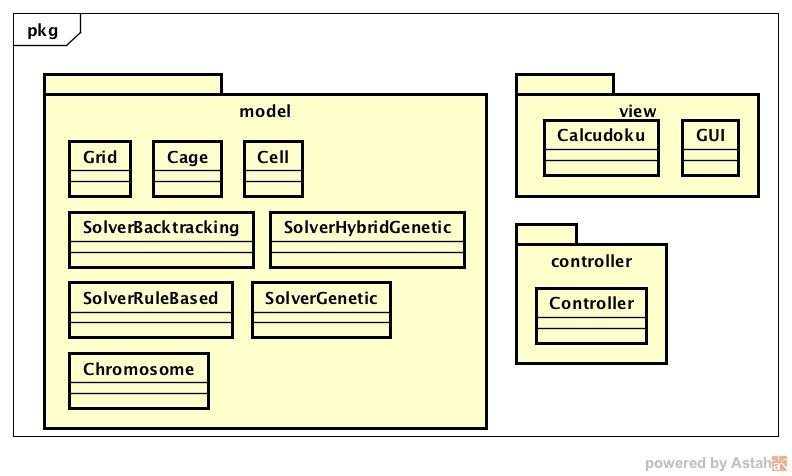
\includegraphics[scale=0.5]{Gambar/Analisis/DiagramKelas.jpg}
\caption[Diagram kelas untuk perangkat lunak permainan teka-teki Calcudoku]{Diagram kelas untuk perangkat lunak permainan teka-teki Calcudoku}
\label{fig:analisiskelas}
\end{figure}

Berdasarkan diagram kelas yang dapat dilihat pada Gambar~\ref{fig:analisiskelas}, kelas-kelas yang digunakan dalam perangkat lunak Calcudoku adalah:

\begin{enumerate}
\item \textit{Package} model, yaitu \textit{package} yang berisi kelas-kelas yang merepresentasikan permainan teka-teki Calcudoku. \textit{Package} ini terdiri dari 8 kelas, yaitu:
	\begin{enumerate}
	\item Kelas Grid, yaitu kelas yang merepresentasikan sebuah \textit{grid} dalam permainan Calcudoku.
	\item Kelas Cell, yaitu kelas yang merepresentasikan sebuah sel dalam \textit{grid}.
	\item Kelas Cage, yaitu kelas yang merepresentasikan sebuah \textit{cage} dalam \textit{grid}.
	\item Kelas SolverBacktracking, yaitu kelas yang merepresentasikan \textit{solver} untuk permainan Calcudoku dengan algoritma \textit{backtracking}.
	\item Kelas SolverHybridGenetic, yaitu kelas yang merepresentasikan \textit{solver} untuk permainan Calcudoku dengan algoritma \textit{hybrid genetic}.
	\item Kelas SolverRuleBased, yaitu kelas yang merepresentasikan \textit{solver} untuk permainan Calcudoku dengan algoritma \textit{rule based}, bagian pertama dari algoritma \textit{hybrid genetic}.
	\item Kelas SolverGenetic, yaitu kelas yang merepresentasikan \textit{solver} untuk permainan Calcudoku dengan algoritma genetik, bagian kedua dari algoritma \textit{hybrid genetic}.
	\item Kelas Chromosome, yaitu kelas yang merepresentasikan sebuah kromosom dalam algoritma genetik.
	\end{enumerate}
\item \textit{Package} view, yaitu \textit{package} yang merepresentasikan GUI untuk permainan Calcudoku. \textit{Package} ini terdiri dari 2 kelas, yaitu:
	\begin{enumerate}
	\item Kelas Calcudoku, yaitu kelas yang merepresentasikan \textit{frame} untuk GUI permainan Calcudoku. Kelas ini berisi menu \textit{bar}, dan panel yang merepresentasikan \textit{grid} untuk permainan Calcudoku (kelas GUI).
	\item Kelas GUI, yaitu kelas yang merepresentasikan \textit{grid} untuk permainan Calcudoku.
	\item Kelas GeneticParameters, yaitu kelas yang berisi \textit{form} untuk mengatur nilai dari parameter-parameter untuk algoritma genetik.
	\end{enumerate}
\item \textit{Package} controller, yaitu penghubung antara kelas-kelas yang ada di dalam \textit{package} model dengan kelas-kelas yang ada di dalam \textit{package} view. \textit{Package} ini terdiri dari 1 kelas, yaitu kelas Controller. Kelas ini menghubungkan kelas-kelas yang ada di dalam  \textit{package} model dengan kelas-kelas yang ada di dalam \textit{package} view.
\end{enumerate}

Penjelasan tentang variabel-variabel dan \textit{method-method} yang ada di dalam kelas-kelas di atas akan dijelaskan di dalam bab Perancangan.

\section{Diagram \textit{Sequence}}
\label{sec:diagramsequence}

Diagram \textit{sequence} adalah diagram yang menggambarkan interaksi antar kelas dalm suatu skenario.

Gambar~\ref{fig:sequenceconstructor} menunjukkan diagram \textit{sequence} saat perangkat lunak dibuka.

\begin{figure}
\centering
\captionsetup{justification=centering}
\includegraphics[scale=0.5]{Gambar/Analisis/SequenceDiagramConstructor.png}
\caption[Diagram \textit{sequence} saat perangkat lunak dibuka]{Diagram \textit{sequence} saat perangkat lunak dibuka}
\label{fig:sequenceconstructor}
\end{figure}

Gambar~\ref{fig:sequenceload} menunjukkan diagram \textit{sequence} saat menu \textit{item} "\textit{Load Puzzle File}" dalam menu "\textit{File}" dipilih.

\begin{figure}
\centering
\captionsetup{justification=centering}
\includegraphics[scale=0.2]{Gambar/Analisis/SequenceDiagramLoad.png}
\caption[Diagram \textit{sequence} saat menu \textit{item} "\textit{Load Puzzle File}" dalam menu "\textit{File}" dipilih]{Diagram \textit{sequence} saat menu \textit{item} "\textit{Load Puzzle File}" dalam menu "\textit{File}" dipilih}
\label{fig:sequenceload}
\end{figure}

Gambar~\ref{fig:sequencefilechooser} menunjukkan diagram \textit{sequence} saat \textit{file} permainan yang ingin dibuka dalam \textit{file chooser} dipilih.

\begin{figure}
\centering
\captionsetup{justification=centering}
\includegraphics[scale=0.3]{Gambar/Analisis/SequenceDiagramFileChooser.png}
\caption[Diagram \textit{sequence} saat \textit{file} yang ingin dibuka dalam \textit{file chooser} dipilih]{Diagram \textit{sequence} saat \textit{file} yang ingin dibuka dalam \textit{file chooser} dipilih}
\label{fig:sequencefilechooser}
\end{figure}

Gambar~\ref{fig:sequenceloadpuzzlefile} menunjukkan diagram \textit{sequence} saat \textit{file} permainan yang sudah dipilih dibuka.

\begin{figure}
\centering
\captionsetup{justification=centering}
\includegraphics[scale=0.4]{Gambar/Analisis/SequenceDiagramLoadPuzzleFile.png}
\caption[Diagram \textit{sequence} saat \textit{file} permainan yang sudah dipilih dibuka]{Diagram \textit{sequence} saat \textit{file} permainan yang sudah dipilih dibuka}
\label{fig:sequenceloadpuzzlefile}
\end{figure}

Gambar~\ref{fig:sequencereset} menunjukkan diagram \textit{sequence} saat menu \textit{item} "\textit{Reset Puzzle}" dalam menu "\textit{File}" dipilih.

\begin{figure}
\centering
\captionsetup{justification=centering}
\includegraphics[scale=0.4]{Gambar/Analisis/SequenceDiagramReset.png}
\caption[Diagram \textit{sequence} saat menu \textit{item} "\textit{Reset Puzzle}" dalam menu "\textit{File}" dipilih]{Diagram \textit{sequence} saat menu \textit{item} "\textit{Reset Puzzle}" dalam menu "\textit{File}" dipilih}
\label{fig:sequencereset}
\end{figure}

\clearpage

Gambar~\ref{fig:sequenceclose} menunjukkan diagram \textit{sequence} saat menu \textit{item} "\textit{Close Puzzle File}" dalam menu "\textit{File}" dipilih.

\begin{figure}
\centering
\captionsetup{justification=centering}
\includegraphics[scale=0.5]{Gambar/Analisis/SequenceDiagramClose.png}
\caption[Diagram \textit{sequence} saat menu \textit{item} "\textit{Close Puzzle File}" dalam menu "\textit{File}" dipilih]{Diagram \textit{sequence} saat menu \textit{item} "\textit{Close Puzzle File}" dalam menu "\textit{File}" dipilih}
\label{fig:sequenceclose}
\end{figure}

Gambar~\ref{fig:sequencecheck} menunjukkan diagram \textit{sequence} saat menu \textit{item} "\textit{Check Puzzle File}" dalam menu "\textit{File}" dipilih.

\begin{figure}
\centering
\captionsetup{justification=centering}
\includegraphics[scale=0.5]{Gambar/Analisis/SequenceDiagramCheck.png}
\caption[Diagram \textit{sequence} saat menu \textit{item} "\textit{Check Puzzle File}" dalam menu "\textit{File}" dipilih]{Diagram \textit{sequence} saat menu \textit{item} "\textit{Check Puzzle File}" dalam menu "\textit{File}" dipilih}
\label{fig:sequencecheck}
\end{figure}

Gambar~\ref{fig:sequencebt} menunjukkan diagram \textit{sequence} saat menu \textit{item} "\textit{Backtracking}" dalam menu "\textit{Solve}" dipilih.

\begin{figure}
\centering
\captionsetup{justification=centering}
\includegraphics[scale=0.4]{Gambar/Analisis/SequenceDiagramBacktracking.png}
\caption[Diagram \textit{sequence} saat menu \textit{item}" \textit{Backtracking}" dalam menu "\textit{Solve}" dipilih]{Diagram \textit{sequence} saat menu \textit{item}" \textit{Backtracking}" dalam menu "\textit{Solve}" dipilih}
\label{fig:sequencebt}
\end{figure}

Gambar~\ref{fig:sequencehg} menunjukkan diagram \textit{sequence} saat menu \textit{item} "\textit{Hybrid Genetic}" dalam menu "\textit{Solve}" dipilih.

\begin{figure}
\centering
\captionsetup{justification=centering}
\includegraphics[scale=0.2]{Gambar/Analisis/SequenceDiagramHybridGenetic.png}
\caption[Diagram \textit{sequence} saat menu \textit{item} "\textit{Hybrid Genetic}" dalam menu "\textit{Solve}" dipilih]{Diagram \textit{sequence} saat menu \textit{item} "\textit{Hybrid Genetic}" dalam menu "\textit{Solve}" dipilih}
\label{fig:sequencehg}
\end{figure}

\clearpage

Gambar~\ref{fig:sequencegaparameters} menunjukkan diagram \textit{sequence} saat menu \textit{item} "\textit{Set Genetic Algorithm Parameters}" dalam menu "\textit{Solve}" dipilih.

\begin{figure}
\centering
\captionsetup{justification=centering}
\includegraphics[scale=0.5]{Gambar/Analisis/SequenceDiagramGeneticParameters.png}
\caption[Diagram \textit{sequence} saat menu \textit{item}" \textit{Set Genetic Algorithm Parameters}" dalam menu "\textit{Solve}" dipilih]{Diagram \textit{sequence} saat menu \textit{item} "\textit{Set Genetic Algorithm Parameters}" dalam menu "\textit{Solve}" dipilih}
\label{fig:sequencegaparameters}
\end{figure}

Gambar~\ref{fig:sequencegaparametersok} menunjukkan diagram \textit{sequence} saat \textit{button} "\textit{OK}" dalam \textit{form} "\textit{Set Genetic Algorithm Parameters}" dalam menu "\textit{Solve}" dipilih.

\begin{figure}
\centering
\captionsetup{justification=centering}
\includegraphics[scale=0.5]{Gambar/Analisis/SequenceDiagramGeneticParametersOK.png}
\caption[Diagram \textit{sequence} saat \textit{button} "\textit{OK}" dalam \textit{form} "\textit{Set Genetic Algorithm Parameters}" dalam menu "\textit{Solve}" dipilih]{Diagram \textit{sequence} saat \textit{button} "\textit{OK}" dalam \textit{form} "\textit{Set Genetic Algorithm Parameters}" dalam menu "\textit{Solve}" dipilih}
\label{fig:sequencegaparametersok}
\end{figure}

Gambar~\ref{fig:sequencegaparameterscancel} menunjukkan diagram \textit{sequence} saat \textit{button} "\textit{Cancel}" dalam \textit{form} "\textit{Set Genetic Algorithm Parameters}" dalam menu "\textit{Solve}" dipilih.

\begin{figure}
\centering
\captionsetup{justification=centering}
\includegraphics[scale=0.5]{Gambar/Analisis/SequenceDiagramGeneticParametersCancel.png}
\caption[Diagram \textit{sequence} saat \textit{button} "\textit{Cancel}" dalam \textit{form} "\textit{Set Genetic Algorithm Parameters}" dalam menu "\textit{Solve}" dipilih]{Diagram \textit{sequence} saat \textit{button} "\textit{Cancel}" dalam \textit{form} "\textit{Set Genetic Algorithm Parameters}" dalam menu "\textit{Solve}" dipilih}
\label{fig:sequencegaparameterscancel}
\end{figure}

Gambar~\ref{fig:sequenceexit} menunjukkan diagram \textit{sequence} saat perangkat lunak ditutup.

\begin{figure}
\centering
\captionsetup{justification=centering}
\includegraphics[scale=0.5]{Gambar/Analisis/SequenceDiagramExit.png}
\caption[Diagram \textit{sequence} saat perangkat lunak ditutup]{Diagram \textit{sequence} saat perangkat lunak ditutup}
\label{fig:sequenceexit}
\end{figure}